\paragraph*{Mixed-disturbance probability map.}
Figure~\ref{fig:attn-prediction} extends the single-resource trajectory to a supplementary mixed-disturbance episode, \texttt{n10\_mix\_all1.0\_\_episode\_03}. It is selected automatically for high bottleneck activity and displays 241 sampled test windows from the Start$\leq5$ mixed-disturbance checkpoint. The three aligned panels retain the future-event labels, model probabilities and absolute probability errors. Visible mismatches include probabilities on resources without a corresponding positive label as well as incomplete coverage of labelled intervals. The probability map is distinct from a thresholded operational report. Its 20 displayed rows contain the 15 evaluation targets and five human context nodes; the 18 buffer rows are omitted for readability. It therefore illustrates where this supplementary model agrees or disagrees with labels; it is not an aggregate performance result for the retained \texttt{dense\_i1} model.
\zhpara{图~\ref{fig:attn-prediction}将单资源轨迹扩展到补充混合扰动episode \texttt{n10\_mix\_all1.0\_\_episode\_03}。该episode按瓶颈活动度自动选择，展示五分钟混合扰动checkpoint的二百四十一个采样测试窗口。三幅图依次保留未来事件标签、预测概率及绝对概率误差，既显示已标注区间的覆盖，也保留无对应正标签资源上的概率响应与覆盖不足。概率图不同于阈值化后的运行报告；显示的二十行包括十五个正式预测目标及五个人员上下文节点，为提高可读性省略十八个缓冲区行。因此，该图用于定位补充模型与标签的一致或偏离位置，不作为保留 \texttt{dense\_i1} 模型的总体性能证据。}
\begin{figure*}[p]
\centering
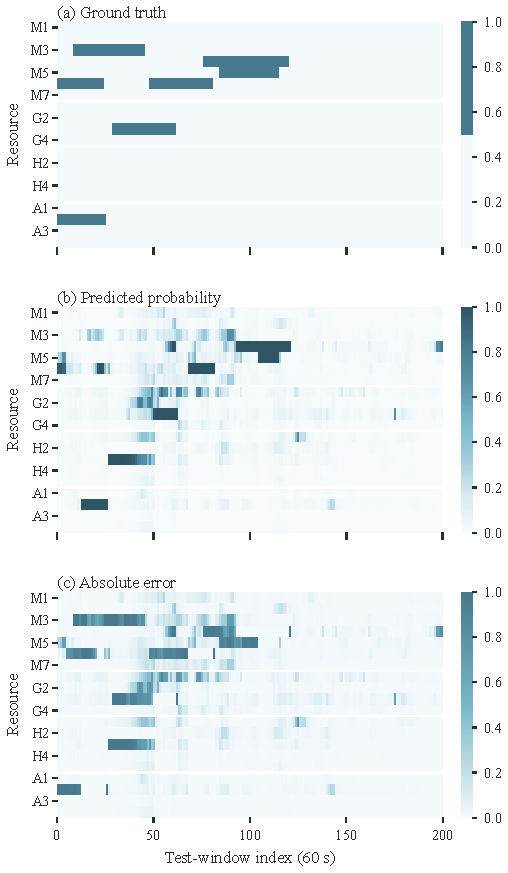
\includegraphics[width=0.98\textwidth,height=0.78\textheight,keepaspectratio]{figures/attention_heatmaps/fig08_prediction_heatmaps.pdf}
\caption{Future-event labels, predicted probabilities and absolute probability errors for the automatically selected high-activity episode \texttt{n10\_mix\_all1.0\_\_episode\_03}. Rows show 20 non-buffer resources and columns 241 sampled test windows; the 18 buffer rows are omitted, and the figure is not a thresholded 15-target report map. Start cap 5 min. Mixed-disturbance supplementary analysis (\texttt{dense\_i1\_mix}, seed 42); not the retained \texttt{dense\_i1} evaluation.}
\label{fig:attn-prediction}
\end{figure*}
